% !TeX root = ../main.tex
% -*- coding: utf-8 -*-

\chapter{绪论}
\label{1}

本章首先阐述深度神经网络模型知识产权保护的研究背景与意义,进而分析相关研究中存在的问题与挑战,然后说明本文的主要工作,最后介绍整篇论文的组织结构与章节安排。

\section{研究背景与意义}

近年来,科技飞速发展,计算资源日益丰富,计算能力得到显著提升,我们正逐渐进入人工智能(Artificial Intelligence, AI)的时代。互联网的快速发展催生了海量数据的产生。深度神经网络(Deep Neural Network, DNN)\cite{samek2021explaining}对数据强大的处理能力,使得DNN已经成为应用最为广泛的人工智能方法之一。自深度神经网络在自然语言处理\cite{wu2023graph,lauriola2022introduction,caucheteux2022brains}、计算机视觉\cite{buhrmester2021analysis,lindsay2021convolutional,gururaj2022deep}、语音识别\cite{dua2022developing}等领域实现突破性应用以来,DNN的应用数量呈爆炸式增长。这些应用已经被被广泛应用于自动驾驶\cite{zhang2022robustness}、癌症检测\cite{shakeel2022automatic}、复杂游戏\cite{ling2020using}等众多场景。在许多领域中,深度神经网络取得了惊人的成就,甚至超越了人类的准确性。

深度神经网络在许多领域都取得了重大的成功,为人类社会生活带来了极大的便利。然而,它也引发了严重的知识产权(Intellectual Property, IP)问题。通常情况下,训练一个大型、高性能的神经网络模型都需要该领域专家的专业知识、规模巨大的数据集以及大量的训练时间和强大的计算资源,具体体现在以下三个方面:

1)人力资源,深度神经网络的设计和优化需要领域专家的专业知识。在设计深度神经网络时,需要考虑多个方面的因素,如网络结构、层数、激活函数等。为了使网络的性能达到最佳水平,需要通过反复试验和调整来设计网络结构和优化网络参数。

2)数据资源,训练数据的获取和处理是深度神经网络训练的第一步。大量的数据是必需的,但这些数据的获取和使用必须遵守相关的法律法规和道德规范。此外,数据的清洗和标注也需要高度的专业知识和劳动力投入。

3)硬件资源,深度神经网络的训练需要漫长的训练时间和大量的计算资源。在训练过程中,需要进行大量的矩阵运算和梯度下降等计算操作,这需要高性能的计算硬件和软件支持。同时,训练时间也可能会很长,需要耐心和耐力。因此,深度神经网络训练需要充足的资源和时间预算,以确保训练过程的顺利进行和最终的成功结果。如GPT-3\cite{brown2020language},包含了1750亿参数,仅训练成本需花费460万美元以上。


因此,高性能的DNN模型是模型所有者知识智慧的结晶,同时需要投入高额的经济成本,模型所有者享有DNN模型的知识产权\cite{wang2021fingerprinting,li2020protecting}。

出于学术目的,模型所有者将DNN模型上传到开源社区。或者,使用机器学习即服务(Machine Learning as a Service, MLaaS)\cite{tanuwidjaja2020privacy}的商业模式,即MLaaS平台通过训练好的DNN模型来向用户提供应用程序接口(Application Programming Interface, API)\cite{ofoeda2019application},用户可以通过支付一定的费用来使用API。或者,训练好的DNN模型将成为像我们日常商品一样的消费品,它们由不同的公司或个人进行训练,由不同的供应商分发,最终由用户消费。这样的方式极大的方便了科研工作者和一般的消费者,但同时也为不法分子对模型发起各种模型窃取攻击\cite{hu2021stealing,yue2021black}提供了可能性。这些攻击可以让不法分子以比训练原始模型低很多的成本复制一个盗窃模型,用于提供自己的服务或者进行相关研究。

\begin{figure}[htbp]%%图,[htbp]是浮动格式
	\centering
	\setlength{\abovecaptionskip}{5mm} %图片标题与图片距离
%	\vspace{-2mm}
%	\setlength{\belowcaptionskip}{-1mm} %调整图片标题与下文距离
	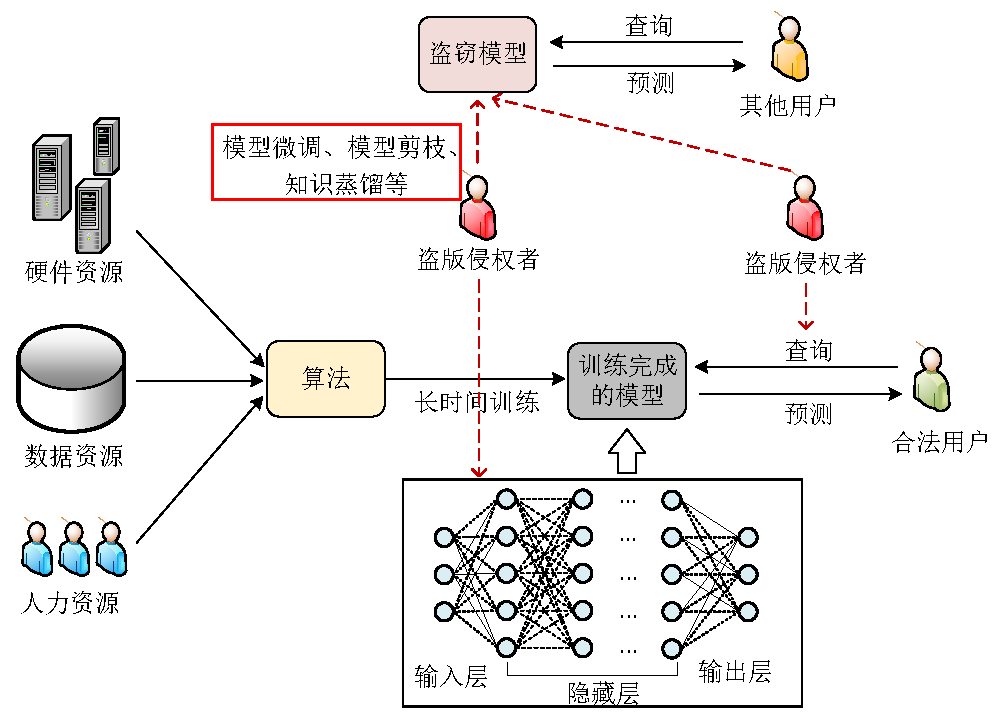
\includegraphics[width=0.97\linewidth]{DNN模型服务和盗窃示意图.pdf}
	\caption{DNN模型服务和盗窃示意图}
	\label{DNN模型服务和盗窃示意图}
%	\vspace{-3mm}  %调整图片标题与下文距离,与\setlength{\belowcaptionskip}{-3mm}等效。
	\end {figure}
	
如图\ref{DNN模型服务和盗窃示意图}所示,模型所有者消耗包括硬件资源、数据资源、人力资源在内的大量资源,经复杂算法进行长时间训练后,发布训练好的模型为合法用户提供服务。然而,盗版侵权者会对模型发起窃取攻击,从而获得一个功能相似的盗窃模型用于自己盈利。主要有两种方式:(1)直接访问原始模型,盗窃后对模型进行修改。(2)在不能直接访问模型时,通过模型提供的服务API进行特定的输入查询,依靠API输出重构模型。

\textbf{模型盗窃方法:}图\ref{DNN模型服务和盗窃示意图}中,不法分子可以通过模型窃取攻击来盗窃模型。主流的模型窃取攻击涉及到对模型的修改,主要包括模型微调\cite{guo2019spottune},模型剪枝\cite{liu2018rethinking},模型压缩\cite{deng2020model}等,简要介绍如下:

1)模型微调:型微调通常用于迁移学习,可以在原始模型的基础上微调模型参数,使模型满足自己的任务需求,同时保持模型的性能。通过微调现有的模型,可以派生出许多功能、结构相似的模型。

2)模型剪枝:模型剪枝是是部署DNN模型的常见方法之一,通过参数修剪来减少DNN的内存需求和计算开销,以便部署到一些资源受限的环境下。然后而模型盗窃者可能会使用修剪来删除水印或指纹。

3)知识蒸馏:模型压缩中常见的方式是知识蒸馏\cite{gou2021knowledge},可以将训练好的模型的知识,蒸馏到其他模型上。这种方式可以更快的训练一个新模型,显著降低模型的训练成本,内存需求和计算开销,同时达到与原始模型接近的性能。研究\cite{hinton2015distilling}表明甚至不需要原始训练数据就可以直接利用API蒸馏模型,因此蒸馏常被用来派生模型。
	
综上所述,如何在训练和部署时保护深度神经网络模型的知识产权是AI领域亟待解决的问题。保护DNN模型知识产权的意义在于确保模型的创造者能够获得其所创造的价值,具体而言,有以下四个方面的意义:

1)保护商业利益:神经网络模型模型通常需要大量的时间、资源和资金才能进行开发和训练。通过保护知识产权,模型的创造者可以确保他们的商业利益得到保护,从而获得他们应得的经济回报。

2)保护创新:神经网络模型模型是创新的产物,保护模型知识产权可以激励更多的人投入到相关研究和开发中。这样可以催生更多的创新,从而推动技术的进步和发展。

3)避免盗用和侵权:保护知识产权可以避免其他人对神经网络模型的盗用和侵权。这些行为可能会导致模型的创造者无法获得应有的经济回报,并可能削弱创造者的商业利益。

4)确保模型质量:通过保护知识产权,模型的创造者可以控制和保证其模型质量。这样可以确保DNN模型在商业应用中的可靠性和有效性,从而提高其商业价值和应用性。


\section{相关研究现状}

神经网络模型作为数字产品,不仅是设计者的知识智慧的结晶,还需要消耗昂贵的计算资源、花费大量的训练时间和海量的训练数据做支撑。近年来,先进模型所带来的工业优势已经被广泛认可,但这也引发了一些不法分子对这些模型进行攻击和窃取。神经网路模型将在未来的信息技术发展中扮演核心角色,因此保护这些模型的重要性显得更加突出。1994年,Van Schyndel等人\cite{van1994digital}首次提出了数字水印的概念,通过将标记隐蔽的嵌入到如音频、视频等数字内容中,来识别其所有权。具体而言,版权所有者通过显示此类标记的存在可以证明其对内容的所有权。由于DNN模型也是一种数字产品,因此,许多研究者从数字媒体水印得到启发,从而设计模型水印和模型指纹用于解决模型的所有权问题。
%\vspace{-3mm}

\subsection{模型水印}

模型水印\cite{GYKJ202207020}是解决神经网络模型知识产权问题的主要方式之一,Uchida等人\cite{uchida2017embedding}在2017年首次提出了在模型中嵌入水印的通用框架。该方法是一种白盒的模式,通过在训练时使用正则化器,这种正则化在参数中引入了所需要的统计偏差来作为嵌入的水印。模型所有者清楚模型内部结构等的细节,并且可以提取嵌入的水印,以此来作为验证模型所有权的依据\cite{zhang2021deep}。
Chen等人\cite{chen2018deepmarks}提出了一种新颖的端到端框架,该框架同时依赖于用户和模型,它需要为每一个用户分配一个代码向量,并将该信息嵌入到可训练权重的的概率密度函数中,同时保持模型的准确性。
为了解决水印易受到歧义攻击的问题,Fan等人\cite{fan2019rethinking}提出了一种在模型中嵌入数字护照的方案,嵌入数字护照的要点是设计和训练DNN模型,使得在伪造护照的情况下,神经网络模型的推断性能显著下降,而真正的护照可以通过查找预定签名来验证。
不同于白盒的模式,另一种黑盒的模式,可以在不访问模型内部的情况下,通过特定的输入输出来验证模型的所有权。
Zhang等人\cite{zhang2018protecting}提出了一种水印植入方法,将水印注入模型。通过扩展神经网络的内在泛化和记忆能力,使得模型能够在训练时学习特意制作的水印,然后在推断时激活预先指定的预测。
Adi等人\cite{adi2018turning}提出了利用模型的后门机制当作DNN模型水印。后门通常是指神经网络模型将输入预测为错误的标签,虽然在大多数情况下这是不可取的,但是却可以将为DNN模型制作水印的任务转化为设计后门的任务。
为了减小水印对模型性能的影响,Le等人\cite{le2020adversarial}提出了一种零比特水印算法,该算法标记模型的操作本身,稍微调整它的决策边界,来使特定的查询得到特定的输出。在减少模型性能损失的同时,该算法可以远程操作模型或API服务,通过少量的查询提取水印。
这些黑盒的方法利用对抗性样本作为触发集,或者使用一组特定的训练样本,然后根据特殊样本的输出来提取水印。因此黑盒的方法在所有权验证中不需要访问模型的权重参数和内部结构。
除此之外,Rouhani等人\cite{rouhani2018deepsigns}提出了一种端到端的IP保护框架DeepSigns,可以在DNN模型中插入连贯的数字水印。DeepSigns引入了一种通用水印方法,不同于直接将水印信息嵌入到模型的权重中,DeepSigns将任意N位字符串嵌入到各层激活集的概率密度函数中,这意味着水印信息嵌入在DNN的动态内容中,并且只能通过特定的输入数据来触发,并且对权重矩阵等静态属性没有影响。

然而,DNN模型水印的嵌入步骤总是会对原始模型进行修改。具体而言,白盒水印修改模型内部,比如模型权重、激活函数、甚至模型架构,而黑盒水印通过特殊的训练调整模型来指定特定的输出。这些修改将会影响DNN模型在原始任务上的性能。除了减少对模型性能的影响,如何减小模型水印的嵌入代价也是模型水印的重要目标。

\subsection{模型指纹}

模型指纹是解决神经网络模型知识产权问题的又一主流方法。不同于模型水印,模型指纹不需要对模型本身进行修改,而是利用模型本身来寻找和提取一些固有的的特征作为模型指纹,一般来说,不会影响模型的性能。

Zhao等人\cite{zhao2020afa}提出了一种针对神经网络分类模型的指纹技术,该技术旨在提取模型本身的固有特征,而不是嵌入额外的水印。具体而言,该方法选择一组专门设计的对抗性样本作为模型指纹特征,称为对抗性标记,相比于其他不相关的模型,它可以更好地从原始模型转移到派生出的模型上。
与Zhao等人\cite{zhao2020afa}的方法类似,Lukas等人\cite{lukas2019deep}提出了一种用于神经网络分类器的指纹识别方法。该方法从源模型中提取一组特殊的输入,以便只有源模型的派生模型在此类输入的分类上与源模型一致。这些输入是可转移对抗性样本的一个子类,它们的目标标签会从源模型转移到其派生模型上。所有者通过验证分类是否一致,判断模型是否从源模型派生。
同样利用分类模型的分类边界,Cao等人\cite{cao2021ipguard}针对DNN分类器提出了一种名叫IPGuard的指纹方法,该方法的关键是分类模型可以由其分类边界唯一的表示。基于这一原理,IPGuard在模型所有者的神经网络模型分类边界上提取了一些数据点,并使用它们对分类器进行指纹识别,如果DNN分类器对大多数指纹数据点预测相同的标签,那么该模型被认为是模型所有者分类器的盗版模型。
除了以上针对分类模型的指纹方法,Li等人\cite{li2021novel}提出了一种适用于生成对抗网络(Generative Adversarial Network, GAN)\cite{goodfellow2020generative}知识产权保护的指纹识别方案。该方案从目标GAN和分类器构建了一个复合深度学习模型,然后从该复合模型中生成隐蔽的指纹样本,并将其注册到分类器中进行有效的所有权验证。
针对模型水印和指纹容易受到最抗性训练攻击,不适用于多出口DNN模型的知识产权验证的问题,Dong等人\cite{dong2021fingerprinting}提出了一种根据推理时间,而不是推理预测的结果来为多出口模型建立指纹的新方法。

然而,模型窃取攻击通常会涉及到对原始模型的修改,作为指纹的固有特征也会受到影响。因此指纹是脆弱的,所有的指纹方法都试图找到可以承受某些修改攻击的强鲁棒性指纹。此外,模型指纹不适用于小样本数据集。对于小样本数据集,由于模型的特征向量可能会存在过拟合或欠拟合的情况,因此可能会导致模型指纹的准确性降低。

\textbf{歧义攻击问题:}虽然模型水印和模型指纹在保护模型知识产权方面已经取得了很大的进展,但除了上述提到的问题外,无论是水印还是指纹都容易受到歧义攻击\cite{fan2019rethinking,li2019piracy}。歧义攻击是指不法分子盗窃模型后,通过为神经网络模型伪造其他水印或指纹来对所有权验证产生干扰。直观地,如果模型盗窃者可以在水印模型上嵌入第二个水印或者提取第二个指纹,那么该模型的所有权归属存在巨大的歧义。


\section{本文主要工作}

为了解决深度神经网络模型的知识产权问题,本文提出了近边界数据,一种分布在分类边界附近的特殊样本。模型指纹\cite{cao2021ipguard}使用对抗性样本抽象地反映模型分类边界,同一组对抗性样本的输入,其引起的决策模式的变化可以用于比较模型知识的相似性。但是这种方法是脆弱的,对模型的任意操作都有可能破坏这种特性。因此,本文不直接比较决策模式的变化,它是不可信任的,而是比较对抗性样本与分类边界的距离。大多数对抗性样本都是位于分类边界附近的,也就是说,它们与分类边界的距离很近。对抗性样本的这种性质被本文所利用并构造近边界数据。经过测试,本文发现绝大多数的模型窃取方法都无法改变这种结果,即使在盗窃模型中样本分类受到影响,其仍然位于分类边界附近。近边界数据背后的意义是如果被用于所有权验证如果两个模型的决策模式相似,参与训练的近边界数据一定可以反映出来。受这个特性的启发,将近边界数据作为水印验证所有权是传统的思路,即使不会对模型的精度造成影响,这样的水印也是脆弱的,很难抵御歧义攻击。因此本文提出由近边界数据驱动的模型所有权推断方法,代替传统的模型水印、指纹验证所有权。

本文方法的主要原理如图\ref{方法原理图}所示,其思想是构造私有的近边界数据,当判断一个模型的所有权时,模型所有者和盗窃者分别提供各自的私有近边界数据,距离分类边界最近的被推断获得所有权。

\begin{figure}[htb]%%图,[htbp]是浮动格式
	\centering
	\setlength{\abovecaptionskip}{5mm} %图片标题与图片距离
	%	\vspace{-2mm}
%	\setlength{\belowcaptionskip}{-3mm} %调整图片标题与下文距离
	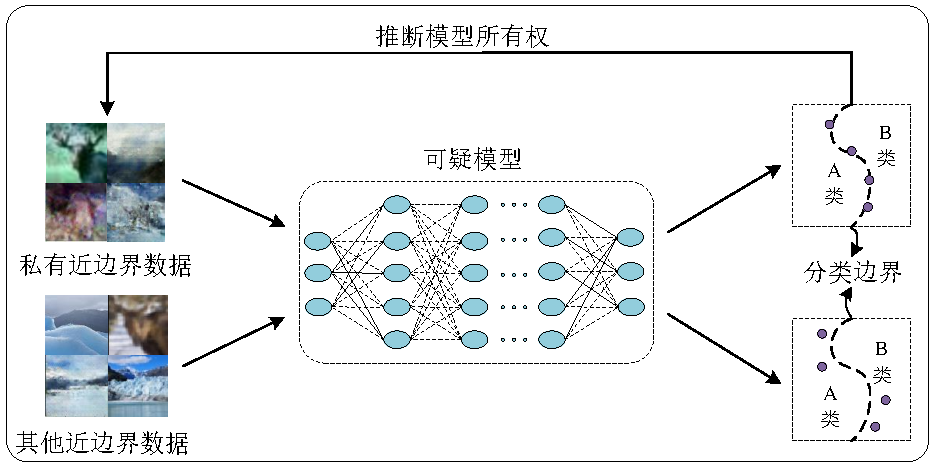
\includegraphics[width=1\linewidth]{方法原理图.pdf}
	\caption{近边界数据推断所有权}
	\label{方法原理图}
	%	\vspace{-3mm}  %调整图片标题与下文距离,与\setlength{\belowcaptionskip}{-3mm}等效。
	\end {figure}

本文的主要工作如下:

1)提出基于数据推断模型所有权的新思路,并利用对抗性样本构造近边界数据以抵御模型窃取攻击。与过去工作中利用模型水印和指纹验证模型所有权相比,使用数据在对应模型上结果作为所有权推断依据,结果的可比性和唯一性可以有效避免歧义攻击。通过实验验证了近边界数据的近边界性可以很好的继承到从源模型派生出的模型上,因此可以作为推断模型所有权的依据。本文利用生成对抗性样本算法生成了初始近边界数据。

2)设计了基于DCGAN的近边界数据特征提取器,用以私有化初始的近边界数据,并且设计了一种新的损失函数用以微调源模型,增加推断模型所有权的置信度。为了防止近边界数据被轻易伪造,本文训练了DCGAN作为数据特征提取器,提取近边界数据特征后,生成新的、私有化的近边界数据。在此基础之上,重新设计了新的损失函数微调源模型,在保持DNN模型性能的情况下,以95\%以上的置信度成功推断模型所有权。

3)基于ResNet18\cite{he2016deep}和三个公开数据集进行了广泛的实验,实验结果证明了近边界数据在推断模型所有权上的显著效果。本文在三个公开数据集上分别训练了ResNet18作为源模型,并且使用模型微调,不同比例模型剪枝,知识蒸馏几种方式派生出盗窃模型,使用VGG11\cite{simonyan2014very}作为无关对照模型。对生成初始近边界数据的方法选择、近边界数据私有化方法的选择、近边界数据的可继承性、源模型微调的影响、模型所有权推断的有效性和近边界数据规模的可伸缩性几个方面对本文提出的方法进行了详细的实验和分析,实验结果证明了基于近边界数据推断模型所有权方法的有效性和鲁棒性。

\section{本文组织架构}

\begin{figure}[htb]%%图,[htbp]是浮动格式
	\centering
		\setlength{\abovecaptionskip}{5mm} %图片标题与图片距离
%	\vspace{-2mm}
%	\setlength{\belowcaptionskip}{-3mm} %调整图片标题与下文距离
	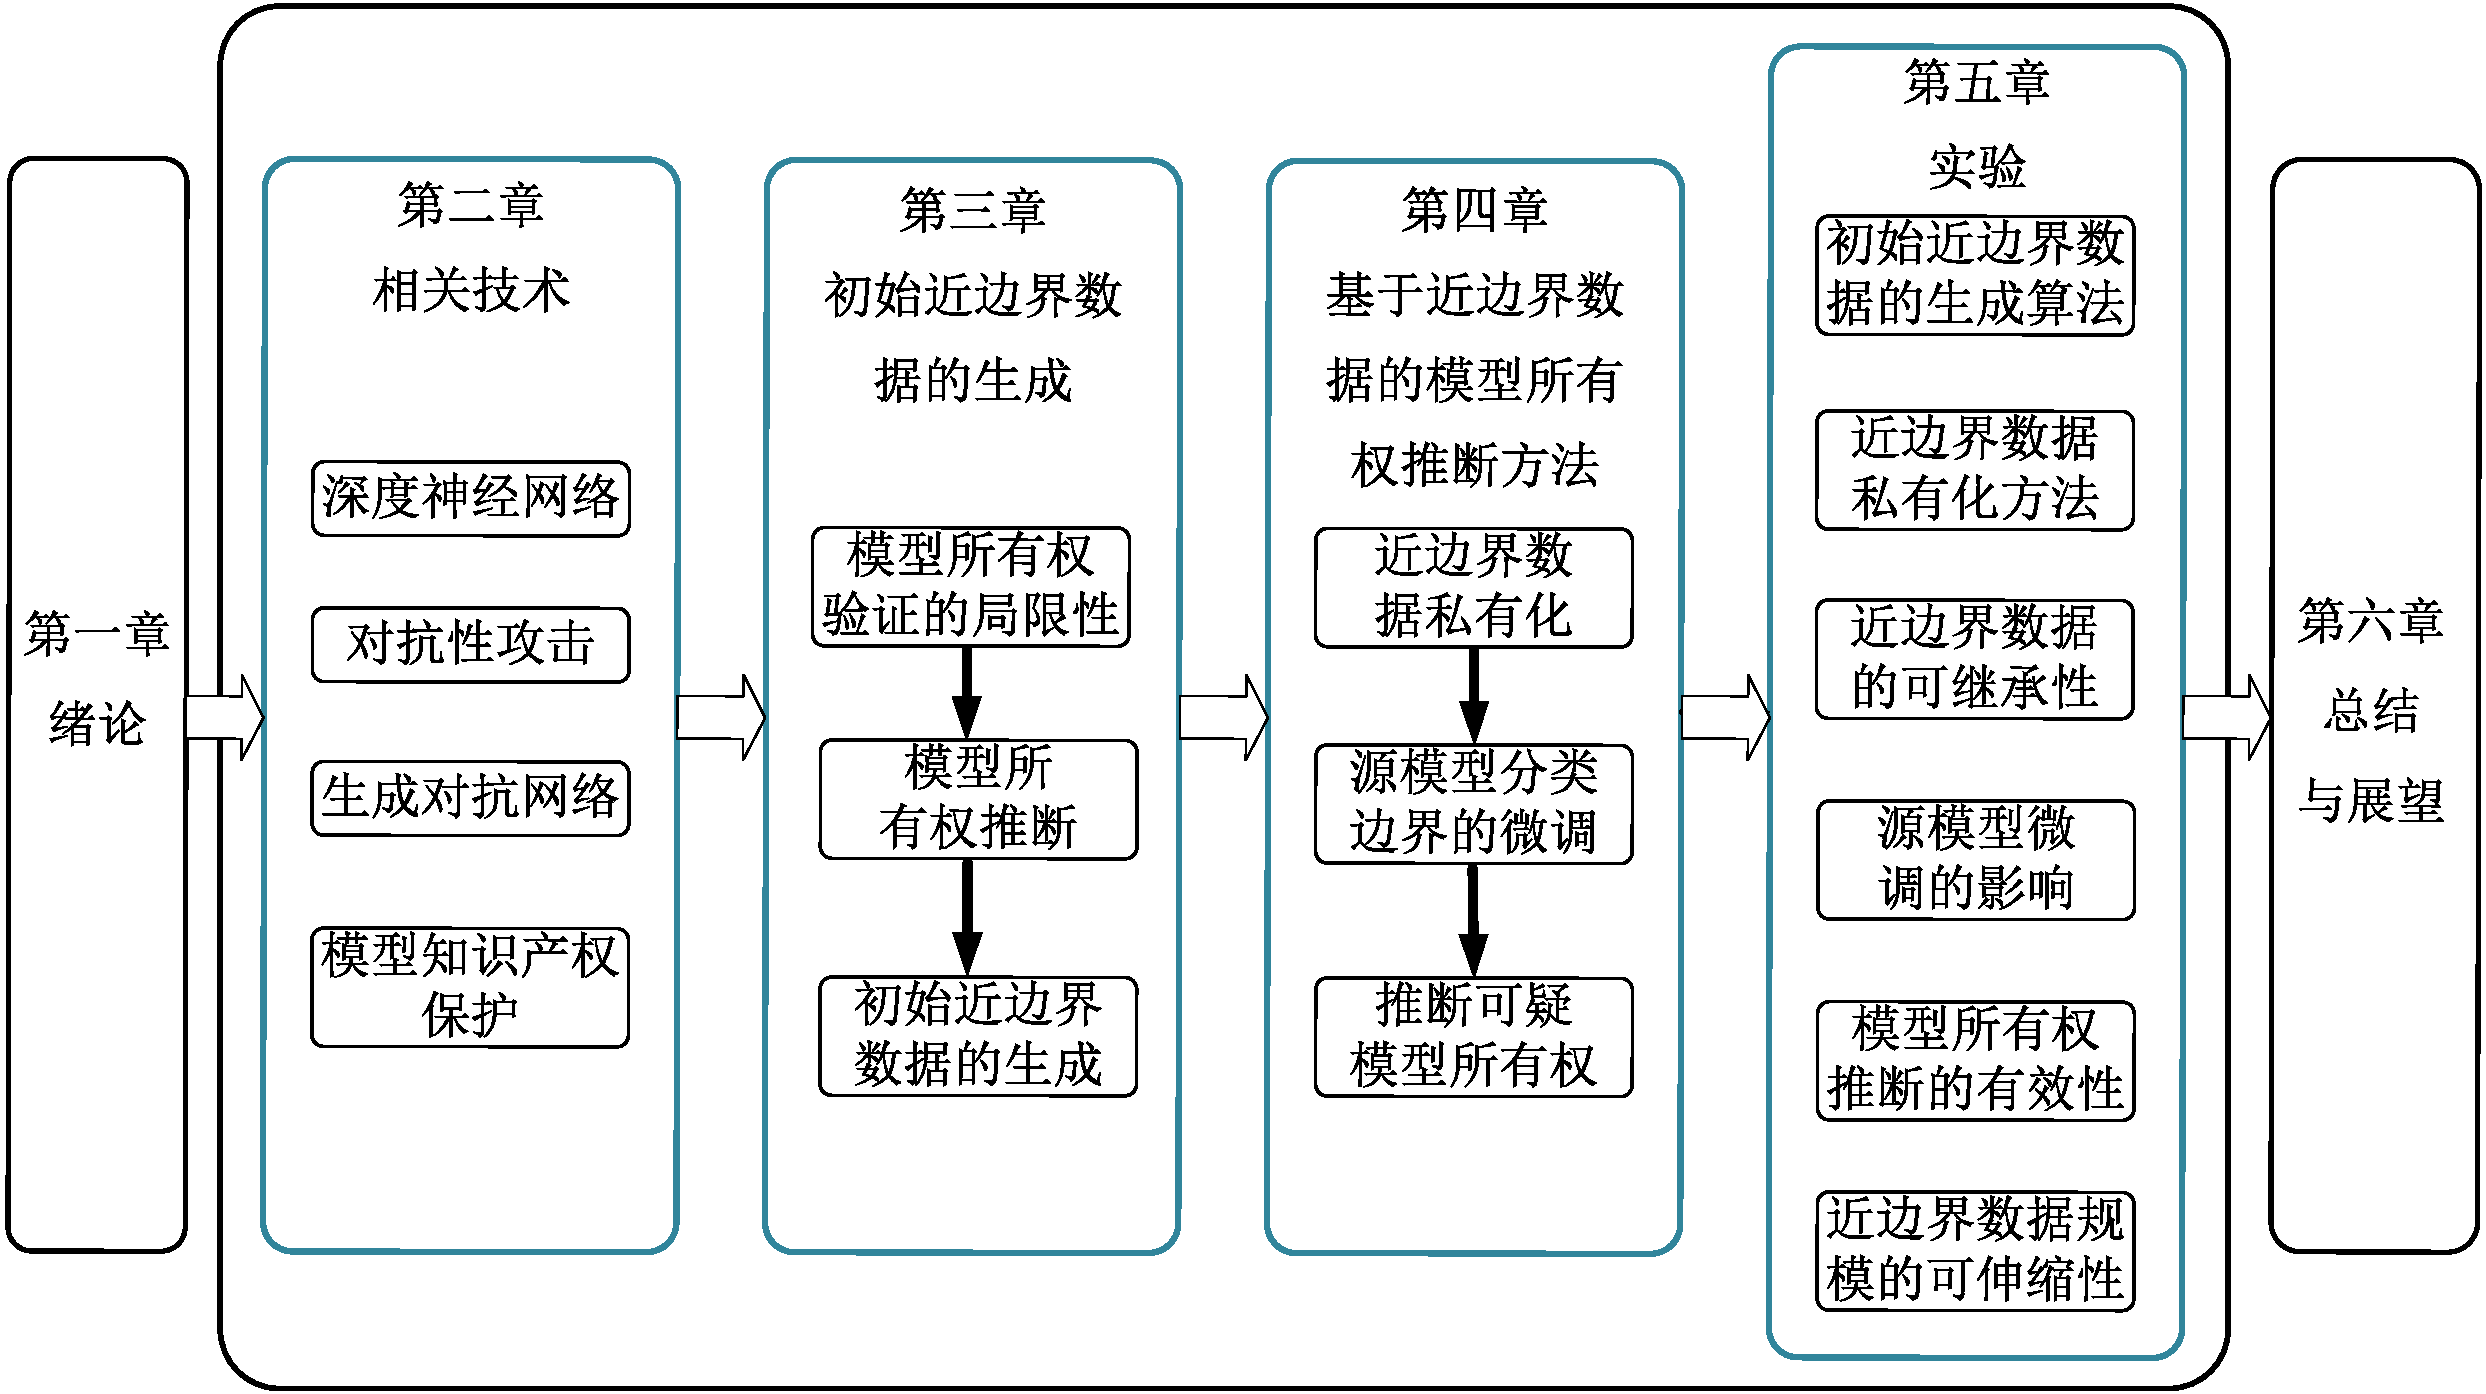
\includegraphics[width=1\linewidth]{章节架构图.pdf}
	\caption{章节架构图}
	\label{章节架构图}
	%	\vspace{-3mm}  %调整图片标题与下文距离,与\setlength{\belowcaptionskip}{-3mm}等效。
	\end {figure}
	
本文对近边界数据进行研究,提出一种基于近边界数据推断模型所有权的方法。本文的组织架构如图\ref{章节架构图}所示,第二章为后面章节提供技术基础。第三章提出模型所有权推断代替所有权验证,解决歧义攻击问题,并生成所有权推断所需的初始近边界数据。第四章在第三章的基础上对初始近边界数据进行初始化,然后基于近边界数据进行所有权推断。第五章对本文提出方法进行全面的测试与评估。全文共分为六各章节,每个章节的主要内容如下:

第一章:绪论。本章首先介绍了神经网络模型在当今时代的广泛应用和研发的昂贵成本,说明了保护DNN模型知识产权的必要性和重大意义,然后介绍了模型水印和模型指纹两种保护方法的研究现状,并针对相关研究存在的问题提出了本文的研究内容,最后简要说明了各个章节的内容安排。

第二章:相关技术。本章首先介绍了深度神经网络基本原理和结构并解释本文使用到的相关术语,然后介绍了对抗性攻击和生成对抗网络的基本原理,最后介绍了模型水印、模型指纹两种知识产权保护方法。为第三章、第四章提供技术基础和理论依据。

第三章:初始近边界数据的生成。本章首先分析了通过传统模型水印、模型指纹来做所有权验证的局限性,然后提出了数据驱动的所有权推断方法。接着研究了近边界数据在源模型和其派生模型上的可继承性,说明近边界数据可用于所有权推断。最后生成了所有权推断所需的初始近边界数据。

第四章:基于近边界数据的模型所有权推断方法。本章首先介绍了需要将初始近边界数据私有化的原因,然后训练生成对抗网络,用其生成器生成新的、私有化的近边界数据。然后设计了新的损失函数微调源模型,使私有近边界数据更加靠近目标分类边界,增加成功推断模型所有权的置信度。最后提出使用假设检验的方法来统计对比结果差异。

第五章:基于近边界数据的模型所有权推断方法分析。本章在ResNet18和三个公开数据集上,对生成初始近边界数据的方法选择、近边界数据私有化方法的选择、近边界数据的可继承性、源模型微调的影响、模型所有权推断的有效性和近边界数据规模的可伸缩性几个方面进行了详细的实验和评估,证明了本文提出方法在推断模型所有权时的有效性和鲁棒性。

第六章:总结与展望。本章总结了全文的工作,分析了本文提出方法在解决模型知识产权问题时的优势与不足,并针对不足之处,提出了未来研究工作的改进方向。
